\documentclass{foi}
\usepackage{lipsum}
\usepackage[utf8]{inputenc}
\usepackage{float}

\lstset{basicstyle=\ttfamily,
  showstringspaces=false,
  commentstyle=\color{red},
  keywordstyle=\color{blue},
}

\vrstaRada{\zavrsni}
\title{Izrada aplikacije za pronalazak termina sastanaka}

\author{Leo Ćavar}
\spolStudenta{\musko}
\mentor{Marko Mijač}
\spolMentora{\musko}
\godina{2024}
\mjesec{Rujan}
\date{2024}
\status{redoviti}
\indeks{0016153823}
\smjer{Informacijski i poslovni sustavi}
\titulaProfesora{Doc. Dr. sc.}

\sazetak{U ovom završnom radu se obrađuje korištenje .NET tehnologija za izradu programa za dogovaranje sastanka. Kroz rad se obrađuje kratko o ASP. NET Core i ASP. NET Web API tehnologijama, kao i koncepte API-ja i HTTP metoda, Google API-ja, uključujući Google Calendar API, autentifikaciju i autorizaciju korisnika pomoću OAuth 2.0 protokola, te primjere zahtjeva za dohvaćanje i upravljanje kalendarskim događajima kroz implementaciju .NET web aplikacije 
}

\kljucneRijeci{API; ASP. NET Core; .NET; C\#; ASP. NET; ; OAuth 2.0; Google Calendar; Google API;}

\begin{document}

\maketitle

\tableofcontents

\pagestyle{plain}
\chapter{Uvod}
U ovom radu ćemo se usredotočiti na izradu programa za dogovaranje sastanaka kroz upotrebu Google API-ja, koji nam omogućava interakciju s iznimno popularnim Google kalendarom. Realizirat ćemo program koristeći ASP.NET Core i Razor stranice za izradu front-end sučelja te upravljanje podacima, dok će ASP.NET Web API služiti za primanje HTTP zahtjeva i komuniciranje s Google servisima za manipuliranje događajima.

\chapter{Metode i tehnike rada}
Za pisanje teksta i formatiranje ovog rada koristio se LaTeX unutar programa Visual Studio Code. Za izradu praktičnog dijela korišten je Visual Studio 2022 i JetBrains Rider.

\chapter{API}
Kada korisnik koristi softver kao klijent, često koristi nekakvo softversko sučelje za interakciju s softverom, ali kada je potrebno da jedan softver koristi dijelove drugog softvera tada koristimo vrstu sučelja za programiranje aplikacija (engl. \textit{Application Programming Interface}) ili skraćeno API.\cite{biehl2015api}
Ta interakcija se najčešće bazira na tome da klijent šalje HTTP zahtjev serveru na određenu lokaciju i dobivaju se nazad podaci.
API zahtjev se sastoji od nekoliko dijelova \cite{altexsoft}
\begin{itemize}
    \item Operacija koja se izvršava (primjer. \textit{GET, POST})
    \item Autentifikacijski parametri
    \item Odredište - URL API završne točke (engl. \textit{endpoint})
\end{itemize}
Poziv može sadržavati i druge parametre ali ovo su tri osnovna koja će se uvijek koristiti.
\section{HTTP zahtjevi}
Kada klijent šalje zahtjev poslužitelju mora specifirati u zahtjevu koju metodu želi izvršiti, imena metoda se odnose na ono što želimo postići sa zahtjevom. \cite{Maurya2021} 
\begin{itemize}
    \item \textbf{GET} metoda se koristi za dohvaćanje podataka
    \item \textbf{POST} - slanje i dodavanje podataka
    \item \textbf{PUT} - Ažuriranje podataka
    \item \textbf{DELETE} - brisanje resursa 
\end{itemize}

\section{RESTFul API}
RESTFul API je vrsta API-ja koja prati REST \textit(eng. {representational state transfer}) principe dizajna, može biti u bilo kojem jeziku i može koristiti bilo koju vrstu podataka \cite{ibm_rest_api}.
Iako najčešće koristi HTTP protokol on nije nužno vezan za njega.\cite{Microsoft2023}
\begin{itemize}
    \item \textbf{Jedinstveno sučelje} - API dizajn mora biti konzistentan i predvidljiv, s pristupom resursima putem standardnih HTTP metoda kao što su GET, POST, PUT i DELETE.
    
    \item \textbf{Razdvajanje klijenta i servera} - Klijent i server su neovisni, gdje server ne čuva informacije o stanju klijenta između zahtjeva, a klijent nema direktan pristup serverovim podatcima.
    
    \item \textbf{Bezustanje (engl. \textit{Stateless})} - Svaki zahtjev od klijenta prema serveru mora sadržavati sve potrebne informacije za obradu, bez potrebe za čuvanjem stanja na serveru.
    
    \item \textbf{Keširanje} - Resursi se mogu keširati kako bi se smanjilo opterećenje servera i omogućilo ponovnu upotrebu već preuzetih podataka.
    
    \item \textbf{Sustav slojeva} - Slojevita arhitektura omogućuje umetanje posrednika između klijenta i servera, dodajući funkcionalnosti poput keširanja ili sigurnosnih provjera.
    
    \item \textbf{Kôd na zahtjev (opcionalno)} - Klijent može preuzeti i izvršiti kod od servera radi proširenja funkcionalnosti aplikacije. 
\end{itemize}

\chapter{ASP.NET Core}
\section{ASP.NET MVC}
ASP.NET MVC je framework koji se bazira na MVC (engl. \textit{Model-View-Controller}) arhitekturi, izgrađen je na .NET platformi i koristi se za izradu web aplikacija \cite{Tyler2024}.
Kao što ime glasi, MVC arhitektura se sastoji od modela, pregleda (eng. \textit{View}) i kontrolera (eng. \textit{Controller}). Ovaj oblik dizajna prati prvi princip SOLID metoda, razdvajanja odgovornosti (eng. \textit{Seperation of concerns}).
MVC omogućava ponovnu upotrebljivost, i zbog podjele na 3 glavne komponente olakšava održavanje koda. \cite{GeeksforGeeks2024}
\begin{figure}[H]
    \centering
    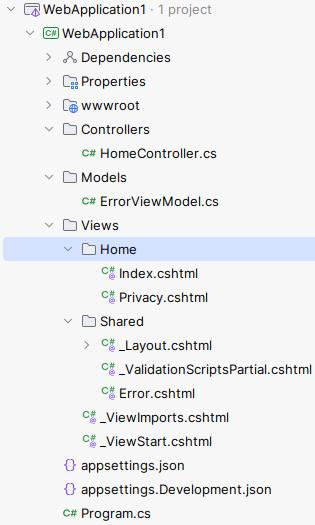
\includegraphics[width=0.6\textwidth]{slike/MVC_project.jpeg}
    \caption{Prikaz MVC u ASP.NET MVC projektu (Izvor: autor)}
    \label{fig:mvc_projekt}
\end{figure}

\subsection{Model}
Unutar konteksta ASP.NET MVC projekta, model predstavlja C\# klasu koja sadrži svojstva za spremanje podataka kojima upravljamo. Model je neovisan o korisničkom sučelju ali često će postojati pregled (engl. textit{View}) koji odgovara za prikaz i upravljanje modelom.
Model također može sadržavati poslovnu logiku za upravljanje podacima, iako to nije učestala praksa i često se ta uloga daje servisima.
\subsection{View}
Pregledi (eng. \textit{Views}) se koriste za prikazivanje podataka i korisničku interakciju. ASP.NET MVC koristi Razor stranice, sa ekstenzijom \textit{cshtml}. Razor stranice omogućavaju pisanje C\# koda unutar HTML datoteka koji služi za interaktiranje sa HTML oznakama za generiranje web sadržaja \cite{Smith2022}. Najčešće će svaki pregled imati svoj kontroler koji je odgovoran za rad s pregledima.
\begin{itemize}
    \item \textbf{Dijelomični pogledi} (engl. \textit{partial views}) omogućuju smanjenje dupliciranja koda upravljanjem ponovljivim dijelovima pogleda. Primjerice, dijelomični pogled je prikladan za biografiju autora na blogu koja se pojavljuje u više pogleda. 
    
    \item \textbf{Komponente pogleda} (engl. \textit{view components}) slične su dijelomičnim pogledima po tome što smanjuju ponavljanje koda, ali su prikladne za sadržaj pogleda koji zahtijeva izvršavanje koda na poslužitelju za generiranje web stranice.
\end{itemize}
\subsection{Controller}
\section{ASP.NET Web API}

\chapter{Zaključak}
.NET okruženje za skriptiranje u GNU/Linux naredbenom retku pruža nove mogućnosti za razvoj i automatizaciju. Kroz rad je demonstriran veći broj Bash i .NET skripti i demonstrirana je integracija .NET alata i Bash ljuske koristeći .NET alat dotnet-shell. Kroz primjere su prikazane prednosti i nedostatci oba sustava. .NET poboljšava interoperabilnost time što se skripte mogu direktno koristiti na svim operacijskim sustavima koji imaju instalirano .NET okruženje. Također, .NET pruža dodatne funkcionalnosti preko svojih biblioteka i NuGet paketa što omogućuje jednostavno razvijanje kompleksnijih skripti čime se još više mogu poboljšati radni procesi. Prednost Bash skripti je što rade na svim GNU/Linux distribucijama koje koriste Bash ljusku bez potrebe za dodatnim instalacijama i zahtjevaju manje resursa od .NET skripti čime su lakše za sustave. Da zaključim, sinergija .NET okruženja i Bash skriptnog jezika u GNU/Linux operacijskom sustavu omogućuje moćno okruženje za projekte automatizacije iz razloga što se može koristiti najbolje od oba jezika pri pisanju skripti, .NET elementi za kompleksne unaprijed pripremljene funkcionalnosti, a Bash za GNU/Linux specifične radnje ukoliko ima potrebe za njima. 


\printbibliography[title=Popis literature]
\addcontentsline{toc}{chapter}{Popis literature}

\listoffigures
\addcontentsline{toc}{chapter}{Popis slika}

\listoftables
\addcontentsline{toc}{chapter}{Popis tablica}

\end{document}
